\begin{frame}
  {Kernfragen dieser Woche}
  \onslide<+->
  \onslide<+->
  \Large
  \centering 
  Verständnis dafür, dass wir bisher nur über \alert{Extensionen} sprechen.\\
  \Halbzeile
  \onslide<+->
  Wissen um Konstruktionen, in denen das nicht ausreicht.\\
  \Halbzeile
  \onslide<+->
  Definition des intensionalen Kalküls auf Basis des extensionalen.\\
  \Halbzeile
  \onslide<+->
  Nochmals zurück zu Chierchia,\\
  weil das entsprechende Kapitel wirklich gut ist.\\
  \onslide<+->
  \Halbzeile
  \grau{\footnotesize Texte für heute: \citealt[Kapitel~5]{ChierchiaMcconnellginet2000} | \citet[Kapitel~5--6]{DowtyEa1981}}
\end{frame}

\section{Wozu Intensionalität?}

\begin{frame}
  {Intensionalität | Beispiele}
  \onslide<+->
  \begin{itemize}[<+->]
    \item \textit{Stockhausen \alert{wird} eine andere Oper schreiben.}
    \item \textit{\alert{Hätte} Arno Schmidt weniger getrunken, \alert{könnte} er noch leben.}
    \item \textit{Gustave Moreau \alert{glaubt}, dass Ästhetizismus toll ist.}
  \end{itemize}
\end{frame}

\begin{frame}
  {Probleme mit Extensionen}
  \onslide<+->
  \onslide<+->
  \begin{itemize}
    \item \grau{\textit{Stockhausen {wird} eine andere Oper schreiben.}}
    \item \grau{\textit{{Hätte} Arno Schmidt weniger getrunken, {könnte} er noch leben.}}
    \item \grau{\textit{Gustave Moreau {glaubt}, dass Ästhetizismus toll ist.}}
  \end{itemize}
  \Halbzeile
  \begin{itemize}[<+->]
    \item \alert{Syntax} der Ausdrücke | Problemlos mit Einführung von Auxiliaren
    \item \alert{Wahrheitsbedingungen} | \rot{Nicht angebbar}
      \begin{itemize}[<+->]
        \item in eindimensionalen Modellen ohne Tempus 
        \item und ohne Modellierung von Möglichkeit und Notwendigkeit\\
          \grau{\footnotesize(Modalverben, modale Adverbiale, \textit{glauben}-Verben)}
      \end{itemize}
  \end{itemize}
\end{frame}


\begin{frame}
  {Was sind Intensionen?}
  \onslide<+->
  \onslide<+->
  \gruen{Extension} (Bedeutung) und \alert{Intension} (Sinn)\\
  \onslide<+->
  \Zeile
  \centering 
  \begin{tabular}{llll}
    \toprule
    \textbf{Synt.\ Typ} & \textbf{Bedeutung} & \textbf{Sinn} & \textbf{Beispiele} \\
    \midrule
    \visible<4->{NP & \gruen<4>{Individuum} & \alert<4>{Individuenkonzept} & \emph{Venus}, \textit{Helmut Kohl}} \\
    \visible<5->{VP & \gruen<5>{Menge von Individuen} & \alert<5>{Eigenschaftskonzept} & \emph{Kolibri}, \textit{laufen}} \\
    \visible<6->{S  & \gruen{Wahrheitswert} & \alert{Proposition} \grau{(Gedanke)} & \emph{Ich mag Kolibris.} }\\
    \bottomrule
  \end{tabular}
\end{frame}

\begin{frame}
  {Intensionen}
  \onslide<+->
  \onslide<+->
  Noch wissen wir nicht viel über Intensionen. Offensichtliche Eigenschaften aber:\\
  \Halbzeile
  \begin{itemize}[<+->]
    \item Nicht rein wahrheitsfunktional\\
      \grau{\footnotesize "`Was ist in der Welt der Fall?"' reicht nicht aus.}
    \item Wissen über die \alert{tatsächlichen}, \alert{vergangenen} und \alert{möglichen} Zustände der Welt\\
      \grau{\footnotesize PSOA = \textit{possible state of affairs}}\\
      \grau{\footnotesize Z.\,B.\ alle vergangenen SOAs; die PSOAs, die Horst Lichter für möglich hält usw.}
    \item Sowas wie \alert{mehrdimensionale Wahrheitsbedingungen}
    \item Vermitteln zwischen Wissen über Dinge und Wahrheitswerten
  \end{itemize}
\end{frame}

\begin{frame}
  {Logik von PSOAs}
  \onslide<+->
  \onslide<+->
  Wir brauchen eine Logik für PSOAs!\\
  \Halbzeile
  \begin{itemize}[<+->]
    \item Offensichtliche \alert{logische Beschränkungen auf PSOAs}
      \Halbzeile
    \item Solche Sätze scheitern nicht nur, weil sie nicht wahr sind:\\
      \alert{\textit{Im Jahr 1985 wird Arno Schmidt planen, "`\textit{Julia}"' bis 1914 fertig zu schreiben.}}
      \Halbzeile
    \item \orongsch{Inkompatibel} mit unserem Wissen über \orongsch{zulässige\slash mögliche PSOAs}
  \end{itemize}
\end{frame}

\begin{frame}
  {Paralleluniversen?}
  \onslide<+->
  \onslide<+->
  \alert{\textit{Maria könnte Arno Schmidt persönlich kennen.}}\\
  \Zeile
  \begin{itemize}[<+->]
    \item Realität | Maria wurde nach dem Tod von AS geboren.
      \Halbzeile
    \item Vorstellbare alternative Realitäten
      \begin{enumerate}[<+->]
        \item AS ist kein Workaholic, trinkt nicht eine Flasche Korn am Tag\\
          und hat daher 1979 keinen Infarkt.
        \item Maria wurde zwanzig Jahre früher geboren.
        \item AS ist von den Toten auferstanden.
        \item \grau{Im Prinzip unbegrenzt viele Möglichkeiten}
      \end{enumerate}
  \end{itemize}
\end{frame}

\section{Formale Modellierung von Intensionen}

\begin{frame}
  {Propositionen und PSOAs}
  \onslide<+->
  \onslide<+->
  Basis der Formalisierung\\
  \Halbzeile
  \begin{itemize}[<+->]
    \item Annahme einer \alert{Menge von PSOAs} (= mögliche Welten)
      \Halbzeile
    \item Jeder PSOA | Exhaustiv bestimmt durch die in ihm wahren Propositionen
      \Halbzeile
    \item Jede Proposition | Zwei-Partitionierung der PSOAs:
      \begin{itemize}[<+->]
        \item Die, in denen sie \alert{wahr} ist
        \item Die, in denen sie \orongsch{falsch} ist
      \end{itemize}
  \end{itemize}
\end{frame}

\begin{frame}
  {Mögliche Welten und Zeiten in Koordinaten}
  \onslide<+->
  \begin{itemize}[<+->]
    \item Für jede \gruen{Proposition} $p_n$ | \gruen{Welten, in der $\dem{p_n}=1$} | \alert{$w\in W$}
    \item Für jeden \gruen{Zeitpunkt} | Ein möglicher Zustand jeder Welt | \alert{$i\in I$}
    \item Also zeitlich geordnete \gruen{Welt-Zeit-Koordinaten} | \alert{$\langle w, i\rangle\in W\times I$}
  \end{itemize}
  \Zeile
  \centering
  \onslide<+->
  \resizebox{0.4\textwidth}{!}{
    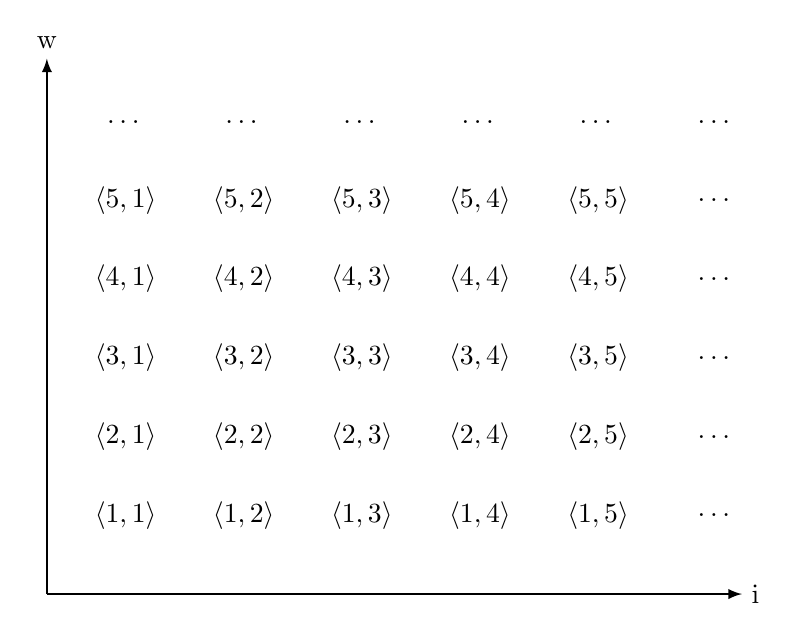
\begin{tikzpicture}

      \node (w) at (0, 7) {w};
      \node (i) at (9, 0) {i};
      \path (0, 0) edge [line width=0.25mm, -latex] (w);
      \path (0, 0) edge [line width=0.25mm, -latex] (i);

      \node [] (w11) at (1, 1) {${\langle 1,1\rangle}$};
      \node [] (w21) at (1, 2) {${\langle 2,1\rangle}$};
      \node [] (w31) at (1, 3) {${\langle 3,1\rangle}$};
      \node [] (w41) at (1, 4) {${\langle 4,1\rangle}$};
      \node [] (w51) at (1, 5) {${\langle 5,1\rangle}$};
      \node [] (w61) at (1, 6) {\ldots};

      \node [] (w12) at (2.5, 1) {${\langle 1,2\rangle}$};
      \node [] (w22) at (2.5, 2) {${\langle 2,2\rangle}$};
      \node [] (w32) at (2.5, 3) {${\langle 3,2\rangle}$};
      \node [] (w42) at (2.5, 4) {${\langle 4,2\rangle}$};
      \node [] (w52) at (2.5, 5) {${\langle 5,2\rangle}$};
      \node [] (w62) at (2.5, 6) {\ldots};

      \node [] (w13) at (4, 1) {${\langle 1,3\rangle}$};
      \node [] (w23) at (4, 2) {${\langle 2,3\rangle}$};
      \node [] (w33) at (4, 3) {${\langle 3,3\rangle}$};
      \node [] (w43) at (4, 4) {${\langle 4,3\rangle}$};
      \node [] (w53) at (4, 5) {${\langle 5,3\rangle}$};
      \node [] (w63) at (4, 6) {\ldots};

      \node [] (w14) at (5.5, 1) {${\langle 1,4\rangle}$};
      \node [] (w24) at (5.5, 2) {${\langle 2,4\rangle}$};
      \node [] (w34) at (5.5, 3) {${\langle 3,4\rangle}$};
      \node [] (w44) at (5.5, 4) {${\langle 4,4\rangle}$};
      \node [] (w54) at (5.5, 5) {${\langle 5,4\rangle}$};
      \node [] (w64) at (5.5, 6) {\ldots};

      \node [] (w15) at (7, 1) {${\langle 1,5\rangle}$};
      \node [] (w25) at (7, 2) {${\langle 2,5\rangle}$};
      \node [] (w35) at (7, 3) {${\langle 3,5\rangle}$};
      \node [] (w45) at (7, 4) {${\langle 4,5\rangle}$};
      \node [] (w55) at (7, 5) {${\langle 5,5\rangle}$};
      \node [] (w65) at (7, 6) {\ldots};

      \node [] (w16) at (8.5, 1) {\ldots};
      \node [] (w26) at (8.5, 2) {\ldots};
      \node [] (w36) at (8.5, 3) {\ldots};
      \node [] (w46) at (8.5, 4) {\ldots};
      \node [] (w56) at (8.5, 5) {\ldots};
      \node [] (w66) at (8.5, 6) {\ldots};
    \end{tikzpicture}
  }
\end{frame}

\begin{frame}
  {Propositionen und Welten}
  \onslide<+->
  \onslide<+->
  Propositionen sind die Intensionen von Formeln bzw.\ Sätzen!\\
  \Halbzeile
  \begin{itemize}[<+->]
    \item Maximal alle Welten für jede Proposition als wahr, permutiert mit allen anderen\\
      \grau{\footnotesize $w_1$: $p_1$ wahr, alle anderen $p_n$ falsch}\\
      \grau{\footnotesize $w_{12}$: $p_1$ und $p_2$ wahr, alle anderen $p_n$ falsch}\\
      \grau{\footnotesize $w_2$: $p_2$ wahr, alle anderen $p_n$ falsch usw.}\\
    \item Exhaustive Charakterisierung eines Satzes | \alert{Alle Welten, in denen er wahr ist}
    \item \gruen{Intension eines Satzes} | \alert{Alle Welten, in denen er wahr ist}
      \Halbzeile
    \item \gruen{Proposition eines Satzes} | \alert{Charakteristische Funktion} der Menge\\
      der \alert{Welten, in denen er wahr ist} \grau{zu den Zeitpunkten, zu denen er wahr ist}
  \end{itemize}
\end{frame}

\begin{frame}
  {Propositionen als Funktionen}
  \onslide<+->
  \onslide<+->
  Propositionen sind \alert{Funktionen $\{0,1\}^{W\times I}$}\\
  \Zeile
  \onslide<+->
  \centering 
  \resizebox{0.4\textwidth}{!}{
    \begin{tikzpicture}

      \node [rectangle, draw, align=left, color=teal, rounded corners=0.5em] (T) at (4.5, 8) {\Huge 1};
      \node [rectangle, draw, align=left, color=orongsch, rounded corners=0.5em] (F) at (3.5, -2) {\Huge 0};

      \node (w) at (0, 7) {w};
      \node (i) at (9, 0) {i};
      \path (0, 0) edge [line width=0.25mm, -latex] (w);
      \path (0, 0) edge [line width=0.25mm, -latex] (i);

      \node [color=teal] (w11) at (1, 1) {${\langle 1,1\rangle}$};
      \node [color=orongsch] (w21) at (1, 2) {${\langle 2,1\rangle}$};
      \node [color=teal] (w31) at (1, 3) {${\langle 3,1\rangle}$};
      \node [color=orongsch] (w41) at (1, 4) {${\langle 4,1\rangle}$};
      \node [color=orongsch] (w51) at (1, 5) {${\langle 5,1\rangle}$};
      \node [color=gray] (w61) at (1, 6) {\ldots};

      \path (w11) edge [line width=0.2mm, -latex, color=teal] (T);
      \path (w21) edge [line width=0.2mm, -latex, color=orongsch] (F);
      \path (w31) edge [line width=0.2mm, -latex, color=teal] (T);
      \path (w41) edge [line width=0.2mm, -latex, color=orongsch] (F);
      \path (w51) edge [line width=0.2mm, -latex, color=orongsch] (F);

      \node [color=orongsch] (w12) at (2.5, 1) {${\langle 1,2\rangle}$};
      \node [color=orongsch] (w22) at (2.5, 2) {${\langle 2,2\rangle}$};
      \node [color=orongsch] (w32) at (2.5, 3) {${\langle 3,2\rangle}$};
      \node [color=orongsch] (w42) at (2.5, 4) {${\langle 4,2\rangle}$};
      \node [color=teal] (w52) at (2.5, 5) {${\langle 5,2\rangle}$};
      \node [color=gray] (w62) at (2.5, 6) {\ldots};

      \path (w12) edge [line width=0.2mm, -latex, color=orongsch] (F);
      \path (w22) edge [line width=0.2mm, -latex, color=orongsch] (F);
      \path (w32) edge [line width=0.2mm, -latex, color=orongsch] (F);
      \path (w42) edge [line width=0.2mm, -latex, color=teal] (T);
      \path (w52) edge [line width=0.2mm, -latex, color=teal] (T);

      \node [color=teal] (w13) at (4, 1) {${\langle 1,3\rangle}$};
      \node [color=orongsch] (w23) at (4, 2) {${\langle 2,3\rangle}$};
      \node [color=teal] (w33) at (4, 3) {${\langle 3,3\rangle}$};
      \node [color=orongsch] (w43) at (4, 4) {${\langle 4,3\rangle}$};
      \node [color=teal] (w53) at (4, 5) {${\langle 5,3\rangle}$};
      \node [color=gray] (w63) at (4, 6) {\ldots};

      \path (w13) edge [line width=0.2mm, -latex, color=teal] (T);
      \path (w23) edge [line width=0.2mm, -latex, color=orongsch] (F);
      \path (w33) edge [line width=0.2mm, -latex, color=teal] (T);
      \path (w43) edge [line width=0.2mm, -latex, color=orongsch] (F);
      \path (w53) edge [line width=0.2mm, -latex, color=teal] (T);

      \node [color=orongsch] (w14) at (5.5, 1) {${\langle 1,4\rangle}$};
      \node [color=teal] (w24) at (5.5, 2) {${\langle 2,4\rangle}$};
      \node [color=teal] (w34) at (5.5, 3) {${\langle 3,4\rangle}$};
      \node [color=orongsch] (w44) at (5.5, 4) {${\langle 4,4\rangle}$};
      \node [color=orongsch] (w54) at (5.5, 5) {${\langle 5,4\rangle}$};
      \node [color=gray] (w64) at (5.5, 6) {\ldots};

      \path (w14) edge [line width=0.2mm, -latex, color=orongsch] (F);
      \path (w24) edge [line width=0.2mm, -latex, color=teal] (T);
      \path (w34) edge [line width=0.2mm, -latex, color=teal] (T);
      \path (w44) edge [line width=0.2mm, -latex, color=orongsch] (F);
      \path (w54) edge [line width=0.2mm, -latex, color=orongsch] (F);

      \node [color=orongsch] (w15) at (7, 1) {${\langle 1,5\rangle}$};
      \node [color=teal] (w25) at (7, 2) {${\langle 2,5\rangle}$};
      \node [color=orongsch] (w35) at (7, 3) {${\langle 3,5\rangle}$};
      \node [color=orongsch] (w45) at (7, 4) {${\langle 4,5\rangle}$};
      \node [color=orongsch] (w55) at (7, 5) {${\langle 5,5\rangle}$};
      \node [color=gray] (w65) at (7, 6) {\ldots};

      \path (w15) edge [line width=0.2mm, -latex, color=orongsch] (F);
      \path (w25) edge [line width=0.2mm, -latex, color=teal] (T);
      \path (w35) edge [line width=0.2mm, -latex, color=orongsch] (F);
      \path (w45) edge [line width=0.2mm, -latex, color=orongsch] (F);
      \path (w55) edge [line width=0.2mm, -latex, color=teal] (T);

      \node [color=gray] (w16) at (8.5, 1) {\ldots};
      \node [color=gray] (w26) at (8.5, 2) {\ldots};
      \node [color=gray] (w36) at (8.5, 3) {\ldots};
      \node [color=gray] (w46) at (8.5, 4) {\ldots};
      \node [color=gray] (w56) at (8.5, 5) {\ldots};
      \node [color=gray] (w66) at (8.5, 6) {\ldots};
    \end{tikzpicture}
  }
\end{frame}


\begin{frame}
  {Überlegen Sie sich das mal \ldots}
  \onslide<+->
  Sind solche Propositionen als Intensionen wirklich \rot{un}befriedigend?\\
  \Halbzeile
  \begin{itemize}[<+->]
    \item Wenn wir den \alert{aktuellen SOA exhaustiv} kennen,\\
      wissen wir für \gruen{jeden Satz, ob er wahr ist}.
      \Halbzeile
    \item Wenn wir wissen, \gruen{welche Sätze wahr sind},\\
      kennen wir den \alert{aktuellen SOA exhaustiv}.
      \Halbzeile
    \item Sätze denotieren Wahrheitswerte, und die Wahrheit eines Satzes\\
      hängt nur vom aktuellem SOA ab.
      \Viertelzeile
    \item[ ] \gruen{Eine Funktion von möglichen Welten zu Wahrheitswerten}\\
      \gruen{charakterisiert daher die Semantik eines Satzes umfassend.}
      \Viertelzeile
    \item Was mehr gäbe es über einen Satz zu wissen?
    \item \orongsch{Sätze mit derselben Intension $\{0,1\}^{W\times I}$ sind absolut gleichbedeutend.}
  \end{itemize}
\end{frame}


\section{Mengen von Welten}

\begin{frame}
  {Implikation und Welten}
  \onslide<+->
  \onslide<+->
  Satzintensionen | Charakteristische Funktionen -- oder \alert{Mengen von $w$ bzw.\ $\langle w,i \rangle$}\\
  \onslide<+->
  \Zeile
  \centering 
  $\alert{p}\rightarrow \gruen{q}$ entspricht $\alert{P}\subseteq \gruen{Q}$:\\
  \Halbzeile
  \onslide<+->
  \resizebox{0.4\textwidth}{!}{
    \begin{tikzpicture}
      \draw[very thick] (0,0) -- (10,0) -- (10,10) -- (0,10) -- cycle;
      \node (W) at (-0.5, 9.5) {$W$};
      \filldraw[black] (6,2) circle (2pt);
      \filldraw[black] (2,1) circle (2pt);
      \filldraw[black] (1,4) circle (2pt);
      \filldraw[black] (2,6) circle (2pt);
      \filldraw[black] (3,4) circle (2pt);
      \filldraw[black] (5,7) circle (2pt);
      \filldraw[black] (6,8) circle (2pt);
      \filldraw[black] (8,4) circle (2pt);
      \filldraw[black] (2,3) circle (2pt);
      \filldraw[black] (9,2) circle (2pt);
      \filldraw[black] (3,1) circle (2pt);
      \filldraw[black] (2,9) circle (2pt);
      \filldraw[black] (4,4) circle (2pt);
      \filldraw[black] (5,6) circle (2pt);
      \filldraw[black] (8,8) circle (2pt);
      \draw[color=blaw, very thick](3,3) circle (1.75);
      \node[color=blaw] (p) at (4.5, 4.5) {$P$};
      \draw[color=gruen, very thick](3.5,3.5) circle (3.1);
      \node[color=gruen] (q) at (6, 6) {$Q$};
    \end{tikzpicture}
  }
\end{frame}

\begin{frame}
  {Synonymie und Welten}
  \onslide<+->
  \onslide<+->
  \centering 
  $\alert{p}\leftrightarrow\gruen{q}$ entspricht $\alert{P}=\gruen{Q}$:\\
  \Halbzeile 
  \onslide<+->
  \resizebox{0.4\textwidth}{!}{
    \begin{tikzpicture}
      \draw[very thick] (0,0) -- (10,0) -- (10,10) -- (0,10) -- cycle;
      \node (W) at (-0.5, 9.5) {$W$};
      \filldraw[black] (6,2) circle (2pt);
      \filldraw[black] (2,1) circle (2pt);
      \filldraw[black] (1,4) circle (2pt);
      \filldraw[black] (2,6) circle (2pt);
      \filldraw[black] (3,4) circle (2pt);
      \filldraw[black] (5,7) circle (2pt);
      \filldraw[black] (6,8) circle (2pt);
      \filldraw[black] (8,4) circle (2pt);
      \filldraw[black] (2,3) circle (2pt);
      \filldraw[black] (9,2) circle (2pt);
      \filldraw[black] (3,1) circle (2pt);
      \filldraw[black] (2,9) circle (2pt);
      \filldraw[black] (4,4) circle (2pt);
      \filldraw[black] (5,6) circle (2pt);
      \filldraw[black] (8,8) circle (2pt);
      \draw[color=blaw, very thick](3,3) circle (1.75);
      \node[color=blaw] (p) at (4.5, 4.5) {$P$};
      \draw[color=gruen, very thick](3,3) circle (1.85);
      \node[color=gruen] (q) at (5, 4) {$Q$};
    \end{tikzpicture}
  }
\end{frame}

\begin{frame}
  {Kontradiktion und Welten}
  \onslide<+->
  \onslide<+->
  \centering 
  Kontradiktion liegt vor bei $\alert{P}\cap\gruen{Q}=0$:\\
  \Halbzeile 
  \onslide<+->
  \resizebox{0.4\textwidth}{!}{
    \begin{tikzpicture}
      \draw[very thick] (0,0) -- (10,0) -- (10,10) -- (0,10) -- cycle;
      \node (W) at (-0.5, 9.5) {$W$};
      \filldraw[black] (6,2) circle (2pt);
      \filldraw[black] (2,1) circle (2pt);
      \filldraw[black] (1,4) circle (2pt);
      \filldraw[black] (2,6) circle (2pt);
      \filldraw[black] (3,4) circle (2pt);
      \filldraw[black] (5,7) circle (2pt);
      \filldraw[black] (6,8) circle (2pt);
      \filldraw[black] (8,4) circle (2pt);
      \filldraw[black] (2,3) circle (2pt);
      \filldraw[black] (9,2) circle (2pt);
      \filldraw[black] (3,1) circle (2pt);
      \filldraw[black] (2,9) circle (2pt);
      \filldraw[black] (4,4) circle (2pt);
      \filldraw[black] (5,6) circle (2pt);
      \filldraw[black] (8,8) circle (2pt);
      \draw[color=blaw, very thick](3,3) circle (1.75);
      \node[color=blaw] (p) at (4.5, 4.5) {$P$};
      \draw[color=gruen, very thick](7,7) circle (2.5);
      \node[color=gruen] (q) at (9, 9) {$Q$};
    \end{tikzpicture}
  }
\end{frame}

\begin{frame}
  {Negation und Welten}
  \onslide<+->
  \onslide<+->
  \centering 
  $\orongsch{\neg}\alert{p}$ entspricht $\orongsch{P/W}$:\\
  \Halbzeile 
  \onslide<+->
  \resizebox{0.4\textwidth}{!}{
    \begin{tikzpicture}
      \filldraw[very thick, black, fill=orongsch!25] (0,0) -- (10,0) -- (10,10) -- (0,10) -- cycle;
      \node (W) at (-0.5, 9.5) {$W$};
      \filldraw[color=blaw, fill=blaw!25, very thick](3,3) circle (1.75);
      \node[color=blaw] (p) at (4.5, 4.5) {$P$};
      \node (PW) at (6.5, 6) {\orongsch{$P/W$}};
      \filldraw[black] (6,2) circle (2pt);
      \filldraw[black] (2,1) circle (2pt);
      \filldraw[black] (1,4) circle (2pt);
      \filldraw[black] (2,6) circle (2pt);
      \filldraw[black] (3,4) circle (2pt);
      \filldraw[black] (5,7) circle (2pt);
      \filldraw[black] (6,8) circle (2pt);
      \filldraw[black] (8,4) circle (2pt);
      \filldraw[black] (2,3) circle (2pt);
      \filldraw[black] (9,2) circle (2pt);
      \filldraw[black] (3,1) circle (2pt);
      \filldraw[black] (2,9) circle (2pt);
      \filldraw[black] (4,4) circle (2pt);
      \filldraw[black] (5,6) circle (2pt);
      \filldraw[black] (8,8) circle (2pt);
    \end{tikzpicture}
  }
\end{frame}


\begin{frame}
  {Modalität = Quantifikation über Welten}
  \onslide<+->
  \onslide<+->
  Was heißt \alert{notwendigerweise} und \alert{möglicherweise}?\\
  \Zeile
  \begin{itemize}[<+->]
    \item \alert{Notwendigkeit}
      \begin{itemize}[<+->]
        \item Es muss so sein, dass $p$.
        \item In allen möglichen\slash denkbaren Welten gilt $p$.
        \item $\alert{\Box p}\equiv \gruen{\forall w\in W}(\orongsch{\den{p}^{w}=1})$ 
      \end{itemize}
      \Halbzeile
    \item \alert{Möglichkeit}
      \begin{itemize}[<+->]
        \item Es kann so sein, dass $p$.
        \item In mindestens einer möglichen\slash denkbaren Welt gilt $p$.
        \item $\alert{\Diamond p}\equiv \gruen{\exists w\in W}(\orongsch{\den{p}^{w}=1})$ 
      \end{itemize}
      \Zeile
    \item \grau{Für alle Wffs $\phi\in Wff$ sind $\Box\phi$ und $\Diamond\phi$ ebenfalls in Wff.}
  \end{itemize}
\end{frame}


\begin{frame}
  {Notwendigkeit als universelle Quantifikation}
  \onslide<+->
  \onslide<+->
  \centering 
  $\alert{\Box p}$ entspricht $\alert{P}=W$:\\
  \Halbzeile 
  \onslide<+->
  \resizebox{0.4\textwidth}{!}{
    \begin{tikzpicture}
      \filldraw[very thick, black, fill=blaw!25] (0,0) -- (10,0) -- (10,10) -- (0,10) -- cycle;
      \node (W) at (-1, 9.5) {$W=\alert{P}$};
      \filldraw[black] (6,2) circle (2pt);
      \filldraw[black] (2,1) circle (2pt);
      \filldraw[black] (1,4) circle (2pt);
      \filldraw[black] (2,6) circle (2pt);
      \filldraw[black] (3,4) circle (2pt);
      \filldraw[black] (5,7) circle (2pt);
      \filldraw[black] (6,8) circle (2pt);
      \filldraw[black] (8,4) circle (2pt);
      \filldraw[black] (2,3) circle (2pt);
      \filldraw[black] (9,2) circle (2pt);
      \filldraw[black] (3,1) circle (2pt);
      \filldraw[black] (2,9) circle (2pt);
      \filldraw[black] (4,4) circle (2pt);
      \filldraw[black] (5,6) circle (2pt);
      \filldraw[black] (8,8) circle (2pt);
    \end{tikzpicture}
  }
\end{frame}

\begin{frame}
  {Möglichkeit als existenzielle Quantifikation}
  \onslide<+->
  \onslide<+->
  \centering 
  $\alert{\Diamond p}$ entspricht $\alert{P}\not=\emptyset$ in $W$ (nur beispielhaft):\\
  \Halbzeile 
  \onslide<+->
  \resizebox{0.4\textwidth}{!}{
    \begin{tikzpicture}
      \draw[black, very thick] (0,0) -- (10,0) -- (10,10) -- (0,10) -- cycle;
      \node (W) at (-0.5, 9.5) {$W$};
      \filldraw[black] (6,2) circle (2pt);
      \draw[color=blaw, dotted, very thick](6,2) circle (0.25);
      \filldraw[black] (2,1) circle (2pt);
      \draw[color=blaw, dotted, very thick](2,1) circle (0.25);
      \filldraw[black] (1,4) circle (2pt);
      \draw[color=blaw, dotted, very thick](1,4) circle (0.25);
      \filldraw[black] (2,6) circle (2pt);
      \draw[color=blaw, dotted, very thick](2,6) circle (0.25);
      \filldraw[black] (3,4) circle (2pt);
      \draw[color=blaw, dotted, very thick](3,4) circle (0.25);
      \filldraw[black] (5,7) circle (2pt);
      \draw[color=blaw, dotted, very thick](5,7) circle (0.25);
      \filldraw[black] (6,8) circle (2pt);
      \draw[color=blaw, dotted, very thick](6,8) circle (0.25);
      \filldraw[black] (8,4) circle (2pt);
      \draw[color=blaw, dotted, very thick](8,4) circle (0.25);
      \filldraw[black] (2,3) circle (2pt);
      \draw[color=blaw, dotted, very thick](2,3) circle (0.25);
      \filldraw[black] (9,2) circle (2pt);
      \draw[color=blaw, dotted, very thick](9,2) circle (0.25);
      \filldraw[black] (3,1) circle (2pt);
      \draw[color=blaw, dotted, very thick](3,1) circle (0.25);
      \filldraw[black] (2,9) circle (2pt);
      \draw[color=blaw, dotted, very thick](2,9) circle (0.25);
      \filldraw[black] (4,4) circle (2pt);
      \draw[color=blaw, dotted, very thick](4,4) circle (0.25);
      \filldraw[black] (5,6) circle (2pt);
      \draw[color=blaw, dotted, very thick](5,6) circle (0.25);
      \filldraw[black] (8,8) circle (2pt);
      \draw[color=blaw, dotted, very thick](8,8) circle (0.25);
      \draw[color=blaw, dotted, very thick](2,3.5) circle (1.5);
      \draw[color=blaw, dotted, very thick](3.5,4) circle (1);
      \draw[color=blaw, dotted, very thick](5,6.5) circle (1);
      \draw[color=blaw, dotted, very thick](5.5,7.5) circle (1);
      \draw[color=blaw, dotted, very thick](6.25,7) circle (2.5);
    \end{tikzpicture}
  }
\end{frame}

\section{Intensionale Modelltheorie}

\begin{frame}
  {Intensionale Modelle}
  \onslide<+->
  \onslide<+->
  Die Modelle werden um Welten $w$ und Zeitpunkte $i$ erweitert.\\
  \Halbzeile
  \begin{itemize}[<+->]
    \item \alert{$\Model=\ram{W,I,<,U,V}$}
      \begin{itemize}[<+->]
        \item \alert{$W$} | Die Menge der Welten
        \item \alert{$I$} | Die Menge der Zeitpunkte\slash Intervalle
        \item \alert{$<$} | Eine Ordnung auf $I$
        \item \alert{$U$} | Die Menge der Individuen\slash Objekte
        \item \alert{$V$} | Eine Auswertungsfunktion für Konstanten jeder Ordnung
      \end{itemize}
      \Halbzeile
    \item Ein Ausdruck $\alpha$ wird jetzt evaluiert relativ zu
      \begin{itemize}[<+->]
        \item Dem Modell \gruen{$\Model$}
        \item Einer \gruen{konkreten Welt} \gruen{$w$}
        \item Einem \gruen{konkreten Zeitpunkt} \gruen{$i$}
        \item Der Belegungsfunktion \gruen{$g$}
          \Halbzeile
        \item \gruen{$\DEMM{\alpha}$}
      \end{itemize}
  \end{itemize}
\end{frame}


\begin{frame}
  {Und Individuen?}
  \onslide<+->
  \onslide<+->
  Individuenkonzepte als Funktionen von Welten zu Individuen\\
  \Halbzeile
  \begin{itemize}[<+->]
    \item \textit{der Präsident der USA}, \textit{der Papst}, \textit{Bond}\\
      \grau{\footnotesize (im Sinn von \textit{der Schauspieler, der gerade Bond spielt)}}
    \item Für \alert{$\beta\in Cons_{ind}$} ist \alert{$V(\beta)$} eine Funktion aus \alert{$U^{W\times I}$}.\\
      \grau{\footnotesize Eine Funktion, die für jedes Welt-Zeit-Paar sagt, wer Präsident, Papst, Bond usw.\ ist.}
  \end{itemize}
  \Halbzeile
  \onslide<+->
  \centering
  \resizebox{0.6\textwidth}{!}{
    \begin{tikzpicture}

      \node (sem) at (-2, 3.5) {\Large\blau{$\dem{\mathbf{Bond}}=$}};
      \node (usw) at (19, 3.5) {\Large\blau{usw.}};

      \node[color=lightgray] (w) at (0, 7) {w};
      \node[color=lightgray] (i) at (9, 0) {i};
      \path[color=lightgray] (0, 0) edge [line width=0.25mm, -latex] (w);
      \path[color=lightgray] (0, 0) edge [line width=0.25mm, -latex] (i);

      \node [] (w11) at (1, 1) [circle, fill, inner sep=2.5pt] {};
      \node [] (w21) at (1, 2) [circle, fill, inner sep=2.5pt] {};
      \node [] (w31) at (1, 3) [circle, fill, inner sep=2.5pt] {};
      \node [] (w41) at (1, 4) [circle, fill, inner sep=2.5pt] {};
      \node [] (w51) at (1, 5) [circle, fill, inner sep=2.5pt] {};
      \node [] (w61) at (1, 6) {\ldots};

      \node [] (w12) at (2.5, 1) [circle, fill, inner sep=2.5pt] {};
      \node [] (w22) at (2.5, 2) [circle, fill, inner sep=2.5pt] {};
      \node [] (w32) at (2.5, 3) [circle, fill, inner sep=2.5pt] {};
      \node [] (w42) at (2.5, 4) [circle, fill, inner sep=2.5pt] {};
      \node [] (w52) at (2.5, 5) [circle, fill, inner sep=2.5pt] {};
      \node [] (w62) at (2.5, 6) {\ldots};

      \node [] (w13) at (4, 1) [circle, fill, inner sep=2.5pt] {};
      \node [] (w23) at (4, 2) [circle, fill, inner sep=2.5pt] {};
      \node [] (w33) at (4, 3) [circle, fill, inner sep=2.5pt] {};
      \node [] (w43) at (4, 4) [circle, fill, inner sep=2.5pt] {};
      \node [] (w53) at (4, 5) [circle, fill, inner sep=2.5pt] {};
      \node [] (w63) at (4, 6) {\ldots};

      \node [] (w14) at (5.5, 1) [circle, fill, inner sep=2.5pt] {};
      \node [] (w24) at (5.5, 2) [circle, fill, inner sep=2.5pt] {};
      \node [] (w34) at (5.5, 3) [circle, fill, inner sep=2.5pt] {};
      \node [] (w44) at (5.5, 4) [circle, fill, inner sep=2.5pt] {};
      \node [] (w54) at (5.5, 5) [circle, fill, inner sep=2.5pt] {};
      \node [] (w64) at (5.5, 6) {\ldots};

      \node [] (w15) at (7, 1) [circle, fill, inner sep=2.5pt] {};
      \node [] (w25) at (7, 2) [circle, fill, inner sep=2.5pt] {};
      \node [] (w35) at (7, 3) [circle, fill, inner sep=2.5pt] {};
      \node [] (w45) at (7, 4) [circle, fill, inner sep=2.5pt] {};
      \node [] (w55) at (7, 5) [circle, fill, inner sep=2.5pt] {};
      \node [] (w65) at (7, 6) {\ldots};

      \node [] (w16) at (8.5, 1) {\ldots};
      \node [] (w26) at (8.5, 2) {\ldots};
      \node [] (w36) at (8.5, 3) {\ldots};
      \node [] (w46) at (8.5, 4) {\ldots};
      \node [] (w56) at (8.5, 5) {\ldots};
      \node [] (w66) at (8.5, 6) {\ldots};

      \draw[very thick](4.75, 3.5) circle (5);
      \node[] (WxI) at (10, 6) {$W\times I$};
      
      \draw[very thick](14, 3) circle (2.5);
      \node[] (U) at (17, 3.5) {$U$};
      
      \node [] (u1) at (14.5, 2) [circle, fill, inner sep=2.5pt] {};
      \node [] (u2) at (12.5, 2.5) [circle, fill, inner sep=2.5pt] {};
      \node [] (u3) at (15.5, 2.75) [circle, fill, inner sep=2.5pt] {};
      \node [] (u4) at (14, 5) [circle, fill, inner sep=2.5pt] {};
      \node [] (u5) at (13.5, 3.5) [circle, fill, inner sep=2.5pt] {};
      \node [] (u6) at (14.5, 2) [circle, fill, inner sep=2.5pt] {};
      \node [] (u7) at (12, 3.25) [circle, fill, inner sep=2.5pt] {};
      \node [] (u8) at (13, 2.5) [circle, fill, inner sep=2.5pt] {};
      \node [] (u9) at (15, 3.5) [circle, fill, inner sep=2.5pt] {};
      \node [] (u10) at (14, 3) [circle, fill, inner sep=2.5pt] {};
      \node [] (u11) at (14, 1.25) {\ldots};

      \path (w11) edge [blaw, very thick,  -latex] (u2);
      \path (w42) edge [blaw, very thick,  -latex] (u2);
      \path (w23) edge [blaw, very thick,  -latex] (u3);
      \path (w15) edge [blaw, very thick,  -latex] (u3);
      \path (w44) edge [blaw, very thick,  -latex] (u4);
      \path (w45) edge [blaw, very thick,  -latex] (u5);
      \path (w55) edge [blaw, very thick,  -latex] (u6);

    \end{tikzpicture}
  }
\end{frame}

\begin{frame}
  {Und Prädikate?}
  \onslide<+->
  \onslide<+->
  Eigenschaftskonzepte als Funktionen von Welten zu Mengen von Tupeln von Individuen\\
  \Halbzeile
  \begin{itemize}[<+->]
    \item Konstanten wie \textit{geht}, \textit{kauft}, \textit{gibt} usw.\ denotieren\\
      unterschiedliche Mengen (bzw.\ CFs) zu unterschiedlichen $\ram{w,i}$-Koordinaten.
    \item Für \alert{$\beta\in Cons_{pred_n}$} ist \alert{$V(\beta)$} eine Funktion aus \alert{$(\wp U^n)^{W\times I}$}.\\
      \grau{\footnotesize Eine Funktion, die für jedes Welt-Zeit-Paar sagt, wer geht, wer was kauft, wer wem was gibt usw.}\\
      \grau{\footnotesize Erinnerung | $U^n=U_1\times U_2\times \cdots\times U_n$}
  \end{itemize}
  \Halbzeile
  \onslide<+->
  \centering 
  \resizebox{0.5\textwidth}{!}{
    \begin{tikzpicture}

      \node (sem) at (-2, 3.5) {\LARGE\blau{$\dem{\mathbf{kauft}}=$}};
      \node (usw) at (28, 3.5) {\LARGE\blau{\ldots}};

      \node[color=lightgray] (w) at (0, 7) {w};
      \node[color=lightgray] (i) at (9, 0) {i};
      \path[color=lightgray] (0, 0) edge [line width=0.25mm, -latex] (w);
      \path[color=lightgray] (0, 0) edge [line width=0.25mm, -latex] (i);

      \node [] (w11) at (1, 1) [circle, fill, inner sep=2.5pt] {};
      \node [] (w21) at (1, 2) [circle, fill, inner sep=2.5pt] {};
      \node [] (w31) at (1, 3) [circle, fill, inner sep=2.5pt] {};
      \node [] (w41) at (1, 4) [circle, fill, inner sep=2.5pt] {};
      \node [] (w51) at (1, 5) [circle, fill, inner sep=2.5pt] {};
      \node [] (w61) at (1, 6) {\ldots};

      \node [] (w12) at (2.5, 1) [circle, fill, inner sep=2.5pt] {};
      \node [] (w22) at (2.5, 2) [circle, fill, inner sep=2.5pt] {};
      \node [] (w32) at (2.5, 3) [circle, fill, inner sep=2.5pt] {};
      \node [] (w42) at (2.5, 4) [circle, fill, inner sep=2.5pt] {};
      \node [] (w52) at (2.5, 5) [circle, fill, inner sep=2.5pt] {};
      \node [] (w62) at (2.5, 6) {\ldots};

      \node [] (w13) at (4, 1) [circle, fill, inner sep=2.5pt] {};
      \node [] (w23) at (4, 2) [circle, fill, inner sep=2.5pt] {};
      \node [] (w33) at (4, 3) [circle, fill, inner sep=2.5pt] {};
      \node [] (w43) at (4, 4) [circle, fill, inner sep=2.5pt] {};
      \node [] (w53) at (4, 5) [circle, fill, inner sep=2.5pt] {};
      \node [] (w63) at (4, 6) {\ldots};

      \node [] (w14) at (5.5, 1) [circle, fill, inner sep=2.5pt] {};
      \node [] (w24) at (5.5, 2) [circle, fill, inner sep=2.5pt] {};
      \node [] (w34) at (5.5, 3) [circle, fill, inner sep=2.5pt] {};
      \node [] (w44) at (5.5, 4) [circle, fill, inner sep=2.5pt] {};
      \node [] (w54) at (5.5, 5) [circle, fill, inner sep=2.5pt] {};
      \node [] (w64) at (5.5, 6) {\ldots};

      \node [] (w15) at (7, 1) [circle, fill, inner sep=2.5pt] {};
      \node [] (w25) at (7, 2) [circle, fill, inner sep=2.5pt] {};
      \node [] (w35) at (7, 3) [circle, fill, inner sep=2.5pt] {};
      \node [] (w45) at (7, 4) [circle, fill, inner sep=2.5pt] {};
      \node [] (w55) at (7, 5) [circle, fill, inner sep=2.5pt] {};
      \node [] (w65) at (7, 6) {\ldots};

      \node [] (w16) at (8.5, 1) {\ldots};
      \node [] (w26) at (8.5, 2) {\ldots};
      \node [] (w36) at (8.5, 3) {\ldots};
      \node [] (w46) at (8.5, 4) {\ldots};
      \node [] (w56) at (8.5, 5) {\ldots};
      \node [] (w66) at (8.5, 6) {\ldots};

      \draw[very thick](4.75, 3.5) circle (5);
      \node[] (WxI) at (10, 6) {\LARGE $W\times I$};
      
      \draw[very thick](17.5,14) circle (2.5);
      \node[] (U) at (20.5,14.5) {\LARGE $U$};
      
      \node [] (u1) at (18,13) [circle, fill, inner sep=2.5pt] {};
      \node [] (u2) at (16,13.5) [circle, fill, inner sep=2.5pt] {};
      \node [] (u3) at (19,13.75) [circle, fill, inner sep=2.5pt] {};
      \node [] (u4) at (18.5, 16) [circle, fill, inner sep=2.5pt] {};
      \node [] (u5) at (19.5,14.5) [circle, fill, inner sep=2.5pt] {};
      \node [] (u6) at (16,13) [circle, fill, inner sep=2.5pt] {};
      \node [] (u7) at (15.5,15.25) [circle, fill, inner sep=2.5pt] {};
      \node [] (u8) at (16.5,13.5) [circle, fill, inner sep=2.5pt] {};
      \node [] (u9) at (18.5,14.5) [circle, fill, inner sep=2.5pt] {};
      \node [] (u10) at (17.5,14) [circle, fill, inner sep=2.5pt] {};
      \node [] (u11) at (17.5,12.25) {\ldots};

      \draw[very thick](17.5, 4) circle (6);
      \node[] (PUxU) at (24.5, 3.5) {\LARGE $\wp(U^2)$};

      \node [] (UxU1a) at (17.5,4) [circle, fill, inner sep=2.5pt] {};
      \node [] (UxU1b) at (18,4) [circle, fill, inner sep=2.5pt] {};
      \node [] (UxU1) at (17.75, 4) [rectangle, draw=black, minimum size=30pt] {};

      \node [] (UxU2a) at (13,3.5) [circle, fill, inner sep=2.5pt] {};
      \node [] (UxU2b) at (13.5,3.5) [circle, fill, inner sep=2.5pt] {};
      \node [] (UxU2) at (13.25, 3.5) [rectangle, draw=black, minimum size=30pt] {};

      \node [] (UxU3a) at (19.5,6) [circle, fill, inner sep=2.5pt] {};
      \node [] (UxU3b) at (20,6) [circle, fill, inner sep=2.5pt] {};
      \node [] (UxU3) at (19.75, 6) [rectangle, draw=black, minimum size=30pt] {};

      \node [] (UxU4a) at (18.5,1) [circle, fill, inner sep=2.5pt] {};
      \node [] (UxU4b) at (19,1) [circle, fill, inner sep=2.5pt] {};
      \node [] (UxU4) at (18.75, 1) [rectangle, draw=black, minimum size=30pt] {};

      \node [] (UxU5a) at (21.25,2) [circle, fill, inner sep=2.5pt] {};
      \node [] (UxU5b) at (21.75,2) [circle, fill, inner sep=2.5pt] {};
      \node [] (UxU5) at (21.5, 2) [rectangle, draw=black, minimum size=30pt] {};

      \node [] (UxU6a) at (14.5,1) [circle, fill, inner sep=2.5pt] {};
      \node [] (UxU6b) at (15,1) [circle, fill, inner sep=2.5pt] {};
      \node [] (UxU6) at (14.75, 1) [rectangle, draw=black, minimum size=30pt] {};

      \node [] (UxU7a) at (17.5,7) [circle, fill, inner sep=2.5pt] {};
      \node [] (UxU7b) at (18,7) [circle, fill, inner sep=2.5pt] {};
      \node [] (UxU7) at (17.75, 7) [rectangle, draw=black, minimum size=30pt] {};

      \node [] (UxU8a) at (16,2.5) [circle, fill, inner sep=2.5pt] {};
      \node [] (UxU8b) at (16.5,2.5) [circle, fill, inner sep=2.5pt] {};
      \node [] (UxU8) at (16.25, 2.5) [rectangle, draw=black, minimum size=30pt] {};

      \draw[lightgray, very thick, -latex] (u1) -- (UxU1a);
      \draw[lightgray, very thick, -latex] (u3) --  (UxU1b);

      \draw[lightgray, very thick, -latex] (u1) -- (UxU3a);
      \draw[lightgray, very thick, -latex] (u2) --  (UxU3b);

      \draw[lightgray, very thick, -latex] (u2) -- (UxU6a);
      \draw[lightgray, very thick, -latex] (u2) --  (UxU6b);

      \draw[lightgray, very thick, -latex] (u6) -- (UxU2a);
      \draw[lightgray, very thick, -latex] (u8) --  (UxU2b);

      \draw[lightgray, very thick, -latex] (u3) -- (UxU5a);
      \draw[lightgray, very thick, -latex] (u7) --  (UxU5b);

      \draw[lightgray, very thick, -latex] (u4) -- (UxU4a);
      \draw[lightgray, very thick, -latex] (u5) --  (UxU4b);

      \node (orousw) at (21, 11) {\LARGE\grau{\ldots}};

      \node [] (PUxU1) at (17.75, 4) [circle, thick, draw=gruen, minimum size=50pt] {};
      \node [] (PUxU2) at (14.5, 2.5) [circle, thick, draw=gruen, minimum size=130pt] {};
      \node [] (PUxU3) at (18.75, 5.5) [circle, thick, draw=gruen, minimum size=150pt] {};
      \node [] (PUxU4) at (17, 3.5) [circle, thick, draw=gruen, minimum size=115pt] {};
      \node [] (PUxU5) at (21.5, 2) [circle, thick, draw=gruen, minimum size=50pt] {};
      \draw[thick, gruen](17.5, 4) circle (5.25);

      \node (grasw) at (17.5, -1) {\LARGE\grau{\ldots}};
      \node (grusw) at (17.5, -1.6) {\LARGE\gruen{\ldots}};
      
      \draw[blaw, very thick, -latex] (w23) --  (PUxU2);
      \draw[blaw, very thick, -latex] (w42) --  (PUxU1);
      \draw[blaw, very thick, -latex] (w31) --  (PUxU4);

    \end{tikzpicture}
  }
\end{frame}

\begin{frame}
  {Auswertung à la Chierchia}
  \onslide<+->
  \onslide<+->
  Diese umständlichen T-Sätze!\\
  \Halbzeile
  \begin{itemize}[<+->]
    \item Wenn \alert{$\beta$} eine Wff der Form \alert{$\delta(t_1,t_2,\cdots,t_n)$} ist
    \Viertelzeile
    \item Dann gilt \alert{$\DEMM{\beta}=1$} gdw
      \begin{itemize}[<+->]
        \item \bl{$\ram{\DEMM{t_1},\DEMM{t_2},\ldots,\DEMM{t_n}}\in\DEMM{\delta}$}
        \item Mit $\DEMM{t_1}=V(\ram{w,i})(t_1)$
      \end{itemize}
      \Halbzeile
    \item[ ] \grau{\footnotesize In einer typentheoretischen Sprache wie $L_{Type}$ wäre Funktionsapplikation möglich.}
  \end{itemize}
\end{frame}

\begin{frame}
  {Quantifikation über Individuen}
  \onslide<+->
  \onslide<+->
  Hier ändert sich eigentlich nichts \ldots\\
  \Halbzeile
  \begin{itemize}[<+->]
    \item Wenn \alert{$\psi$} eine Wff der Form \alert{$\forall x\phi$} ist
    \Viertelzeile
    \item Dann gilt \alert{$\DEMM{\psi}=1$} gdw
      \begin{itemize}[<+->]
        \item Für alle \alert{$u\in U$} \alert{$\Dem{\phi}{\mMm,w,i,g[u/x]}=1$}
      \end{itemize}
      \Viertelzeile
    \item Und Paralleles für den Existenzquantor
  \end{itemize}
\end{frame}

\begin{frame}
  {Auswertung von Modalität}
  \onslide<+->
  \onslide<+->
  Die modalen Funktoren quantifizieren wie gesagt über Welten \ldots\\
  \Halbzeile
  \onslide<+->
  \begin{itemize}[<+->]
    \item<1-> Wenn \alert{$\psi$} eine Wff der Form \alert{$\Box x\phi$} ist
      \Viertelzeile
    \item Dann gilt \alert{$\DEMM{\psi}=1$} gdw
      \begin{itemize}[<+->]
        \item Für alle \alert{$w^{\prime}\in W$}
        \item Und alle \alert{$i^{\prime}\in I$}
        \item \alert{$\Dem{\phi}{\mMm,w^{\prime},i^{\prime},g}=1$}
      \end{itemize}
      \Viertelzeile
    \item Und Paralleles für den \blau{$\Diamond$}-Operator mit Existenzquantifikation
  \end{itemize}
\end{frame}


\begin{frame}
  {Eine Ähnlichkeit zwischen $\forall$ und $\Box$}
  \onslide<+->
  \onslide<+->
  \alert{Modale Möglichkeit} distribuiert wie Allquantifikation \ldots\\
  \Halbzeile
  \begin{itemize}[<+->]
    \item Weil \alert{$\forall x\ekm{P(x)\rightarrow Q(x)}\vdash\ekm{\forall xP(x) \rightarrow \forall x Q(x)}$}\\
      \grau{\footnotesize aber nicht umgekehrt}
    \item Gilt auch \alert{$\Box\ekm{\psi\rightarrow\phi}\vdash\ekm{\Box \psi\rightarrow\Box\phi}$}\\
      \grau{\footnotesize aber nicht umgekehrt}
  \end{itemize}
\end{frame}

\begin{frame}
  {Einige Implikationen und Äquivalenzen}
  \onslide<+->
  \onslide<+->
  Beweistheorie für Modalllogik ist nicht so richtig trivial.\\
  \Viertelzeile
  Hier nur einige interessante Implikationen und Äquivalenzen \ldots\\
  \Halbzeile
  \onslide<+->
  \centering 
  \begin{tabular}[h]{lll}
    \toprule
                           & \textbf{Existenzquantor}                                     & \textbf{Allquantor} \\
    \midrule
    \textbf{Notwendigkeit} & \alert<4>{$\exists x\Box P(x)\rightarrow\Box\exists x P(x)$}%
                           & \alert<6>{$\forall x\Box P(x)\leftrightarrow\Box\forall x P(x)$} \\
    \textbf{Möglichkeit}   & \alert<5>{$\exists x\Diamond P(x)\leftrightarrow\Diamond\exists x P(x)$}%
                           & \alert<7>{$\forall x\Diamond P(x)\rightarrow\Diamond\forall x P(x)$} \\
    \bottomrule
  \end{tabular}
  \Halbzeile
  \begin{itemize}[<+->]
    \item<4-> \alert<4>{\footnotesize Wenn es ein $x$ gibt, dass notwendigerweise $P$ ist,\\
      dann ist es notwendigerweise der Fall, dass es ein $x$ gibt, dass $P$ ist.}
    \item<5-> \alert<5>{\footnotesize Wenn es ein $x$ gibt, dass möglicherweise $P$ ist,\\
      dann ist es möglicherweise der Fall, dass es ein $x$ gibt, dass $P$ ist. Und umgekehrt!}
    \item<6-> \orongsch{\footnotesize Carnap-Barcan-Formel} \alert<6>{\footnotesize Wenn alle $x$ notwendigerweise $P$ ist,\\
      dass ist es notwendigerweise der Fall, dass alle $x$ $P$ sind. Und umgekehrt!} 
    \item<7-> \alert<7>{\footnotesize Wenn alle $x$ möglicherweise $P$ sind,\\
      dann ist es möglicherweise der Fall, dass alle $x$ $P$ sind.}
  \end{itemize}
\end{frame}

